
%---------------------------------------------------------------------------%
\frame{
\frametitle{Continuous Uniform Distribution}
A random variable X is called a continuous uniform random variable over the interval $(a,b)$ if it's probability density function is given by
\[ f(x) = { 1 \over b-a} \hspace{1cm} \mbox{ when } a \leq x \leq b \mbox{     (otherwise } f(x) = 0 ) \]
The corresponding cumulative density function is
\[ F(x) = P(X \leq x) = { x-a \over b-a} \hspace{1cm} \mbox{ when } a \leq x \leq b\]
}
%----------------------------------------------------------------------------------------------------%
\begin{frame}
\frametitle{The Continuous Uniform Distribution}

\vspace{-0.5cm}

\begin{center}
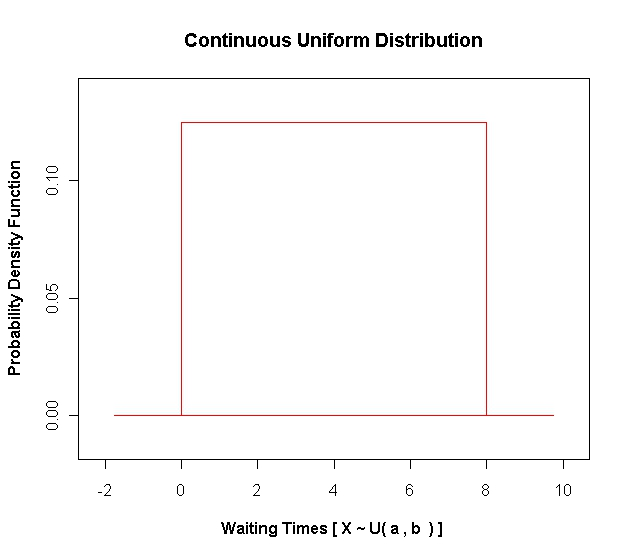
\includegraphics[scale=0.35]{images/6AUniform}

\end{center}
\end{frame}
%---------------------------------------------------------------------------%
\frame{
\frametitle{Continuous Uniform Distribution}
\begin{itemize}
\item The continuous uniform distribution is very simple to understand and implement, and is commonly used in computer applications (e.g. computer simulation).
\item It is also known as the `Rectangle Distribution' for obvious reasons.
\item We specify the word ``continuous" so as to distinguish it from it's discrete equivalent: the discrete uniform distribution.
\item Remark; the dice distribution is a discrete uniform distribution with lower and upper limits 1 and 6 respectively.
\end{itemize}
}
%-----------------------------------------------------%
\frame{
\frametitle{Uniform Distribution Parameters}


The continuous uniform distribution is characterized by the following parameters

\begin{itemize}
\item The lower limit $a$
\item The upper limit $b$
\item We denote a uniform random variable $X$ as $X \sim U(a,b)$
\end{itemize}

It is not possible to have an outcome that is lower than $a$ or larger than $b$.

\[ P(X \leq a) = P(X \geq b) = 0\]
}

%------------------------------------------------------------------------%
\frame{\frametitle{Interval Probability}

\begin{itemize}
\item We wish to compute the probability of an outcome being within a range of values.
\item We shall call this lower bound of this range $L$ and the upper bound $ U$.
\item Necessarily $L$ and $U$ must be possible outcomes.
\item The probability of $X$ being between $L$ and $U$ is denoted $P( L \leq X \leq U )$.

\[
P( L \leq X \leq U ) = { U - L \over b - a}
\]
\item (This equation is based on a definite integral).
\end{itemize}
}

%---------------------------------------------------------------------------------------------------------%
\frame{
\frametitle{Uniform Distribution: Cumulative Distribution}
\begin{itemize}

\item For any value ``c" between the minimum value a and the maximum
value $b$, we can say
\item $P(X \geq c)$ \[P(X \geq c) = {b-c \over b-a}\]
here $b$ is the upper bound while $c$ is the lower bound
\item $P(X \leq c)$ \[P(X \leq c) = {c-a \over b-a}\]
here $c$ is the upper bound while $a$ is the lower bound.
\end{itemize}
}

%-----------------------------------------------------------------------------%
\frame{
\frametitle{Uniform Distribution: Mean and Variance}
\begin{itemize}
\item The mean of the continuous uniform distribution, with parameters $a$ and $b$ is
\[ E(X) = {a+b \over 2}\]
\item The variance is computed as
\[ V(X) = {(b-a)^2 \over 12}\]
\end{itemize}
}
%------------------------------------------------------------------------%
\frame{
\frametitle{Uniform Distribution: Example}

\begin{itemize}
\item Suppose there is a platform in a subway station in a large large city. \item Subway trains arrive \textbf{every three minutes} at this platform. \item What is the shortest possible time a passenger would have to wait for a train?
\item What is the longest possible time a passenger will have to wait?
\end{itemize}

}


%------------------------------------------------------------------------%
\frame{
\frametitle{Uniform Distribution: Example}

\begin{itemize}
 \item What is the shortest possible time a passenger would have to wait for a train?
%\begin{itemize}
\item If the passenger arrives just before the doors close, then the waiting time is zero.
\[ a = 0 \mbox{ minutes } = 0 \mbox{ seconds }  \]
\end{itemize}
}


%------------------------------------------------------------------------%
\frame{
\frametitle{Uniform Distribution: Example}

\begin{itemize}
\item What is the longest possible time a passenger will have to wait?
%\begin{itemize}
\item If the passenger arrives just after the doors close, and missing the train, then he or she will have to wait the full three minutes for the next one.
\[ b = 3 \mbox{ minutes }  = 180 \mbox{ seconds}  \]
\end{itemize}
%\end{itemize}

}

%------------------------------------------------------------------------%
\frame{
\frametitle{Uniform Distribution: Example}

\begin{itemize}
\item What is the probability that he will have to wait longer than 2 minutes?
\[ P(X \geq 2)  = {3-2 \over 3-0} = {1/3} = 0.33333   \]
\item See next slide (shaded area is 1/3 of rectangle)
\end{itemize}
%\end{itemize}

}

%----------------------------------------------------------------------------------------------------%
\begin{frame}
\frametitle{The Continuous Uniform Distribution}

\vspace{-0.5cm}

\begin{center}
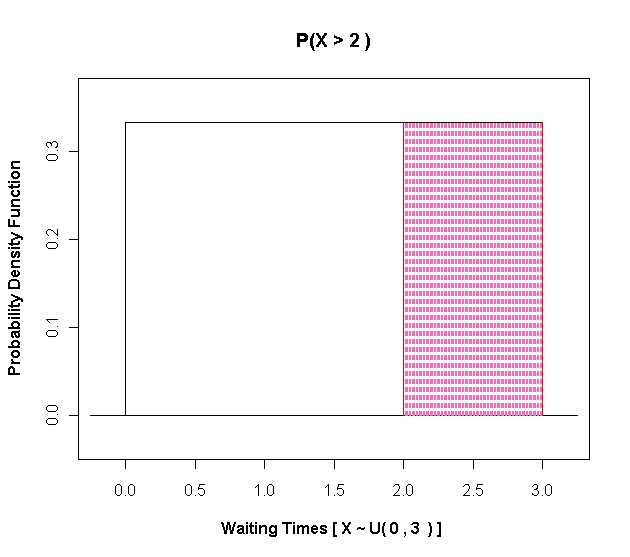
\includegraphics[scale=0.35]{images/6AUniform4}

\end{center}
\end{frame}
%------------------------------------------------------------------------%
\frame{
\frametitle{Uniform Distribution: Example}

\begin{itemize}
\item What is the probability that he will have to wait less than than 45 seconds (i.e. 0.75 minutes)?
\[ P(X \leq 0.75)  = {0.75 - 0 \over 3-0} = {0.75/3} = 0.250  \]

\item See next slide (shaded area is 1/4 of rectangle)
\end{itemize}
%\end{itemize}

}



%----------------------------------------------------------------------------------------------------%
\begin{frame}
\frametitle{The Continuous Uniform Distribution}

\vspace{-0.5cm}

\begin{center}

\end{center}
\end{frame}
%------------------------------------------------------------------------%
\frame{
\frametitle{Uniform Distribution: Expected Value}

We are told that, for waiting times,  the lower limit $a$ is 0, and the upper limit $b$ is 3 minutes. \\ \bigskip The expected waiting time $\textrm{E}[X]$ is computed as follows
\vspace{0.1cm}
\[
\textrm{E}[X] = {b + a \over 2} =  {3 + 0  \over 2}  = 1.5 \mbox{ minutes }
\]

}
%------------------------------------------------------------------------%
\frame{\frametitle{Uniform Distribution: Variance}

The variance of the continuous uniform distribution, denoted $\textrm{V}[X]$,  is  computed using the following formula
\vspace{0.1cm}
\[
\textrm{V}[X] = {(b - a)^2 \over 12}
\]
\vspace{0.1cm}
For our previous example this is
\[
\textrm{V}[X] = {(3 - 0)^2 \over 12} =  {3^2 \over 12} = {9 \over 12} = 0.75
\]
}
\begin{frame}[fragile]
\frametitle{Continuous Distributions: Current Status}
\begin{itemize}
\item (The Continuous Uniform Distribution, Not examinable)
\item The Exponential Distribution (Examinable for midterm)
\item (Exponential Distribution is the Cut-off point for Mid-Term 1)
\item The Normal Distribution
\item The Standard Normal (Z) Distribution.
\item Applications of Normal Distribution
\end{itemize}
\end{frame}

\begin{frame}[fragile]
\frametitle{Exponential Distribution}
The Exponential Distribution may be used to answer the following questions:
\begin{itemize}
\item How much time will elapse before an earthquake occurs in a given region?
\item How long do we need to wait before a customer enters our shop?
\item How long will it take before a call center receives the next phone call?
\item How long will a piece of machinery work without breaking down?
\end{itemize}
\end{frame}

\begin{frame}[fragile]
\frametitle{Exponential Distribution}

\begin{itemize}
\item All these questions concern the time we need to wait before a given event occurs. If this waiting time is unknown, it is often appropriate to think of it as a random variable having an exponential distribution.
\item Roughly speaking, the time $X$ we need to wait before an event occurs has an exponential distribution if the probability that the event occurs during a certain time interval is proportional to the length of that time interval.

\end{itemize}
\end{frame}

%------------------------------------------------------------------------%
\begin{frame}[fragile]
\frametitle{Probability density function}
The probability density function (PDF) of an exponential distribution is

\[
f(x) = \begin{cases}
\lambda e^{-\lambda x}, & x \ge 0, \\
0, & x < 0.
\end{cases}\]
The parameter $\lambda$  is called \textbf{\emph{rate}} parameter.
\end{frame}

%------------------------------------------------------------------------%
\begin{frame}[fragile]
\frametitle{Cumulative density function}
The cumulative distribution function (CDF) of an exponential distribution is

\[
P(X \leq x) = F(x) = \begin{cases}
1-e^{-\lambda x}, & x \ge 0, \\
0, & x < 0.
\end{cases}\]


The complemeent of the CDF (i.e. $P(X \geq x)$ is

\[
P(X \geq x) = \begin{cases}
e^{-\lambda x}, & x \ge 0, \\
0, & x < 0.
\end{cases}\]
\end{frame}

%------------------------------------------------------------------------%
\begin{frame}[fragile]
\frametitle{Expected Value and Variance}
The expected value of an exponential random variable $X$ is:

\[
E[X] = \frac{1}{\lambda}\]
The variance of an exponential random variable $X$ is:

\[
V[X] = \frac{1}{\lambda^2}\]

\end{frame}

%------------------------------------------------------------------------%
\begin{frame}[fragile]
\frametitle{Exponential Distribution: Example}
Assume that the length of a phone call in minutes is an exponential random variable $X$ with parameter
$\lambda = 1/10$. If someone arrives at a phone booth just before you arrive, find the probability that you
will have to wait \begin{itemize}
\item[(a)] less than 5 minutes,
\item[(b)] between 5 and 10 minutes.
\end{itemize}
\end{frame}



%%------------------------------------------------------------------------%
%\begin{frame}[fragile]
%\frametitle{Exponential Distribution: Example}
%\begin{verbatim}
%> dexp(0:10,rate=0.10)
% [1] 0.10000000 0.09048374 0.08187308 0.07408182 0.06703200 0.06065307
% [7] 0.05488116 0.04965853 0.04493290 0.04065697 0.03678794
%>
%> pexp(0:10,rate=0.10)
% [1] 0.00000000 0.09516258 0.18126925 0.25918178 0.32967995 0.39346934
% [7] 0.45118836 0.50341470 0.55067104 0.59343034 0.63212056
%\end{verbatim}
%\end{frame}

%------------------------------------------------------------------------%
\begin{frame}[fragile]
\frametitle{Exponential Distribution: Example}

\begin{itemize}
\item[(a)] $P(X \leq 5)$ = 0.39346934
\item[(b)] $P(5 \leq X \leq 10)$ \\ = $P( X \leq 10) - P( X \leq 5)$ \\ = 0.6321- 0.3934 \\ = 0.2386 \\= 23.86 $\%$
\item[(c)] Alternative approach to (b)\\$P(5 \leq X \leq 10)$ \\ = $P( X \geq 5) - P( X \geq 10)$ \\
= $e^{-0.5} - e^{-1}$
=0.6065 - 0.3678\\
= 0.2386 = 23.86 $\%$
\end{itemize}

\end{frame}



%------------------------------------------------------------------------%
\begin{frame}[fragile]
\frametitle{Exponential Distribution}
\begin{itemize}
\item The Exponential Rate
\item Related to the Poisson mean (m)
\item If we expect 12 occurrences per hour - what is the rate?
\item We would expected to wait 5 minutes between occurrences.
\end{itemize}
\end{frame}

